\documentclass[aspectratio=169, 10pt]{beamer}

% --- Theme and Color Settings ---
\usetheme{Madrid}
\usecolortheme{default}

\definecolor{IITBlue}{RGB}{0,102,204}
\definecolor{IITLightBlue}{RGB}{204,229,255}
\definecolor{IITDarkBlue}{RGB}{0,51,102}
\definecolor{AccentRed}{RGB}{204,0,0}

\setbeamercolor{palette primary}{bg=IITBlue,fg=white}
\setbeamercolor{palette secondary}{bg=IITDarkBlue,fg=white}
\setbeamercolor{palette tertiary}{bg=black,fg=white}
\setbeamercolor{titlelike}{parent=palette primary}
\setbeamercolor{item}{fg=IITBlue}
\setbeamercolor{block title}{bg=IITDarkBlue, fg=white}
\setbeamercolor{block body}{bg=IITLightBlue!30}

% --- Packages ---
\usepackage{graphicx}
\usepackage{amsmath}
\usepackage{booktabs}
\usepackage{tikz}
\usetikzlibrary{shapes,arrows,positioning,calc,fit,backgrounds}
\usepackage{pgfplots}
\pgfplotsset{compat=1.18}


% --- Title Page ---
\title[Quant Research Terminal]{India NLP Quant Research Terminal:\\ A News-Driven Stock Trading System}
\author{Aditi Gupta \and Siddhi Pogakwar \and Anamika Godara \and Shubh Sahu}
\institute[IIT Mandi]{Indian Institute of Technology Mandi}
\date{\today}

\begin{document}

% 1. Title Slide
\begin{frame}
    \titlepage
\end{frame}

% Outline
\begin{frame}{Outline}
    \tableofcontents[hideallsubsections]
\end{frame}

% 2. Literature Survey
\section{Literature Survey}
\begin{frame}{Literature Survey (1/2): Foundational Research}
    \textbf{Base Paper:} \textit{Sustainable Portfolio Construction via Machine Learning: ESG, SDG and Sentiment} (Feng et al., 2024, European Financial Management).
    
    \vspace{0.5em}
    \begin{block}{The Core Idea of the Paper}
        \begin{itemize}
            \item \textbf{The Problem:} Traditional ESG ratings from providers (like MSCI or Bloomberg) are slow, inconsistent, and update only once a year.
            \item \textbf{The Solution:} The authors built a dynamic, daily scoring system using \textbf{Natural Language Processing (NLP)}.
            \item \textbf{The Goal:} To prove that investors can build portfolios prioritizing ESG and Sustainable Development Goals (SDGs) \textit{without} sacrificing financial profit, by using real-time news sentiment.
        \end{itemize}
    \end{block}
\end{frame}

\begin{frame}{Literature Survey (2/2): Methodology \& Our Adaptation}
    \begin{columns}[T]
        \begin{column}{0.48\textwidth}
            \begin{block}{Methodology of Feng et al.}
                \begin{itemize}
                    \item Scraped daily news for S\&P 500 and STOXX 600 stocks.
                    \item Used NLP to create daily scores for Sentiment, ESG, and SDG.
                    \item Applied \textbf{Machine Learning} (Random Forests, Neural Networks) to predict returns.
                    \item Used monthly portfolio optimization, outperforming equal-weight benchmarks.
                \end{itemize}
            \end{block}
        \end{column}
        \begin{column}{0.48\textwidth}
            \begin{block}{How Our Project Adapts This}
                \begin{itemize}
                    \item \textbf{Market Shift:} We brought this methodology to the \textbf{Indian Market} (NIFTY 50), which behaves differently than US/EU markets.
                    \item \textbf{Model Shift:} We used \textbf{FinBERT} (specifically trained on finance) instead of generic NLP.
                    \item \textbf{Risk Engine:} We introduced \textbf{Mean-Semivariance} to protect against downside crashes specifically.
                \end{itemize}
            \end{block}
        \end{column}
    \end{columns}
\end{frame}

% 3. Team Contributions
\section{Team Contributions}
\begin{frame}{Team Contributions}
    \small
    \begin{table}[]
        \centering
        \renewcommand{\arraystretch}{1.4}
        \begin{tabular}{@{}p{2.8cm} p{10.5cm}@{}}
        \toprule
        \textbf{Team Member} & \textbf{Contribution} \\ \midrule
        \textbf{Aditi Gupta}     & \textbf{Data \& NLP}: Collected news articles, removed duplicates, integrated FinBERT for sentiment scoring. \\
        \textbf{Siddhi Pogakwar} & \textbf{Machine Learning}: Built the ML engine to learn how news scores predict future stock returns. \\
        \textbf{Anamika Godara}  & \textbf{Quant Strategy}: Designed portfolio optimization, HMM regime detection, and backtesting logic. \\
        \textbf{Shubh Sahu}      & \textbf{Architecture \& UI}: Built the React frontend, backend server, and system integration. \\ \bottomrule
        \end{tabular}
    \end{table}
\end{frame}

% 2. Introduction
\section{Introduction}
\begin{frame}{Introduction: What Are We Doing?}
    \begin{itemize}
        \item \textbf{Core Idea:} Stock prices move because of real-world news — earnings reports, contracts, scandals.
        \item \textbf{Our Project:} We built an automated system that reads financial news, decides if it is Good or Bad, and automatically trades Indian stocks (NSE/BSE) based on that judgment.
        \item \textbf{Why it matters:} Only large institutions have the infrastructure to read thousands of articles instantly. We built a tool that does this automatically at research scale.
    \end{itemize}
\end{frame}

% 3. Problem Statement
\section{Problem Statement}
\begin{frame}{Problem Statement}
    \begin{block}{The Information Overload}
        Thousands of financial news articles are published every day. A human trader cannot process them fast enough to act.
    \end{block}
    \vspace{0.4em}
    \textbf{Three Core Problems:}
    \begin{enumerate}
        \item \textbf{Junk News:} How do we ignore irrelevant headlines and keep only market-moving articles?
        \item \textbf{Scoring:} How does a computer decide if an article is Positive (+100) or Negative (-100)?
        \item \textbf{Trading Rules:} Even with a positive score, how much money should we allocate without excessive risk?
    \end{enumerate}
\end{frame}

% 4. Objectives
\section{Objectives}
\begin{frame}{Objectives: How We Solve It}
    \begin{enumerate}
        \item \textbf{Collect Data:} Automatically scrape Indian financial news and market prices.
        \item \textbf{Filter \& Score (NLP):} Use AI to discard junk news and assign a Sentiment Score to real news.
        \item \textbf{Predict (ML):} Use 6 months of historical data to predict how much a stock will move based on its score.
        \item \textbf{Manage Risk:} Use mathematical optimization to spread money safely across stocks.
    \end{enumerate}
\end{frame}

% 5. Data Used
\section{Data Used}
\begin{frame}{The Data We Used}
    \begin{columns}[T]
        \begin{column}{0.48\textwidth}
            \begin{block}{Text Data (News)}
                \begin{itemize}
                    \item \textbf{Source:} The Economic Times.
                    \item \textbf{Timeframe:} 2022 -- 2025.
                    \item \textbf{Volume:} 100,000+ headlines.
                    \item \textbf{Cleaning:} Deduplication scripts to avoid double-counting the same article.
                \end{itemize}
            \end{block}
        \end{column}
        \begin{column}{0.48\textwidth}
            \begin{block}{Market Data (Numbers)}
                \begin{itemize}
                    \item \textbf{Source:} Yahoo Finance.
                    \item \textbf{Universe:} NIFTY 50 stocks.
                    \item \textbf{Tracked:} Daily closing prices.
                    \item \textbf{Fundamentals:} P/E ratio, ROE, Debt/Equity for quality filtering.
                \end{itemize}
            \end{block}
        \end{column}
    \end{columns}
\end{frame}

% 6a. Data Preprocessing
\section{Data Preprocessing}
\begin{frame}{Data Preprocessing (1/2): Cleaning \& Mapping}
    \begin{columns}[T]
        \begin{column}{0.48\textwidth}
            \begin{block}{Step 1: Deduplication (MD5 Hash)}
                \begin{itemize}
                    \item Same article copy-pasted across 20+ sites.
                    \item Scores all 20 copies $\Rightarrow$ inflates score by $20\times$.
                    \item MD5 fingerprint computed for each headline.
                    \item Duplicate within 48 hrs $\Rightarrow$ \textbf{dropped}.
                \end{itemize}
            \end{block}
        \end{column}
        \begin{column}{0.48\textwidth}
            \begin{block}{Step 2: Entity Mapping}
                \begin{itemize}
                    \item AI reads English, not stock tickers.
                    \item Dictionary in \texttt{config.py} maps names to tickers.
                    \item \texttt{"RIL"} $\rightarrow$ \texttt{RELIANCE}
                    \item \texttt{"Mukesh Ambani"} $\rightarrow$ \texttt{RELIANCE}
                    \item \texttt{"JLR"} $\rightarrow$ \texttt{TATAMOTORS}
                    \item No match found $\Rightarrow$ article \textbf{dropped}.
                \end{itemize}
            \end{block}
        \end{column}
    \end{columns}
\end{frame}

% 6b. Data Preprocessing
\begin{frame}{Data Preprocessing (2/2): Alignment \& Normalisation}
    \begin{columns}[T]
        \begin{column}{0.48\textwidth}
            \begin{block}{Step 3: Timezone \& Market Alignment}
                \begin{itemize}
                    \item Market hours: 9:15 AM -- 3:30 PM IST.
                    \item News at 9 PM Tuesday $\Rightarrow$ market reacts Wednesday.
                    \item All timestamps converted to IST.
                    \item Post-market news $\rightarrow$ next trading day open.
                    \item Weekend news $\rightarrow$ Monday open.
                \end{itemize}
            \end{block}
        \end{column}
        \begin{column}{0.48\textwidth}
            \begin{block}{Step 4: Text Normalisation}
                \textbf{Before:} {\scriptsize \texttt{<b>TCS Q3 FY25: PAT up 12\% QoQ \#Earnings http://x.co</b>}}\\[4pt]
                \textbf{After:} {\scriptsize \texttt{TCS Q3 FY 2025: Profit After Tax up 12\% Quarter on Quarter}}\\[4pt]
                \begin{itemize}
                    \item Strip HTML tags \& URLs.
                    \item Expand abbreviations (QoQ, PAT, FY25).
                    \item Remove hashtags \& emojis.
                \end{itemize}
            \end{block}
        \end{column}
    \end{columns}
\end{frame}

% 7. AI Models
\section{Our AI Models}
\begin{frame}{The AI Models We Used}
    \small
    \begin{table}[]
        \centering
        \renewcommand{\arraystretch}{1.5}
        \begin{tabular}{@{}p{3cm} p{2.5cm} p{7.5cm}@{}}
        \toprule
        \textbf{Job} & \textbf{Model} & \textbf{Why this model} \\ \midrule
        Filter junk news    & \textbf{DeBERTa}  & Zero-shot classifier; no labelled finance data needed. \\
        Score sentiment     & \textbf{FinBERT}  & Pre-trained on finance text; knows ``downgrade'' = bad. \\
        Predict returns     & \textbf{Ridge/RF} & Handles small, noisy financial datasets without overfitting. \\
        Optimise portfolio  & \textbf{Markowitz}& Proven math to maximise profit for minimum risk. \\ \bottomrule
        \end{tabular}
    \end{table}
\end{frame}

% 8. System Flow
\section{System Flow}
\begin{frame}{End-to-End System Flow}
    \begin{center}
    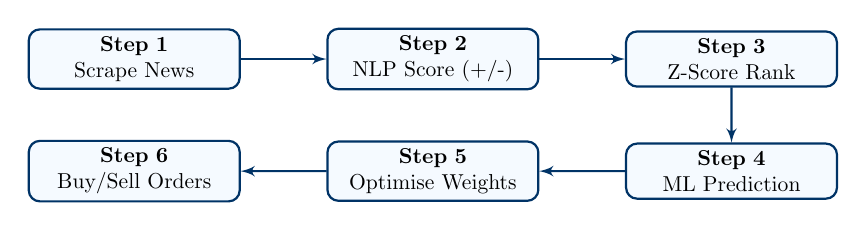
\begin{tikzpicture}[
        auto, thick, scale=0.78, transform shape,
        node distance=1.8cm,
        process/.style={rectangle, draw=IITDarkBlue, fill=IITLightBlue!20, rounded corners,
                        minimum height=2.4em, text width=3.2cm, align=center},
        arrow/.style={draw, -latex', thick, IITDarkBlue}
    ]
        \node[process] (data)    {\textbf{Step 1}\\ Scrape News};
        \node[process, right=1.4cm of data]    (nlp)    {\textbf{Step 2}\\ NLP Score (+/-)};
        \node[process, right=1.4cm of nlp]     (zscore) {\textbf{Step 3}\\ Z-Score Rank};
        \node[process, below=0.9cm of zscore]  (ml)     {\textbf{Step 4}\\ ML Prediction};
        \node[process, left=1.4cm  of ml]      (opt)    {\textbf{Step 5}\\ Optimise Weights};
        \node[process, left=1.4cm  of opt]     (trade)  {\textbf{Step 6}\\ Buy/Sell Orders};
        \path[arrow] (data)   -- (nlp);
        \path[arrow] (nlp)    -- (zscore);
        \path[arrow] (zscore) -- (ml);
        \path[arrow] (ml)     -- (opt);
        \path[arrow] (opt)    -- (trade);
    \end{tikzpicture}
    \end{center}
\end{frame}

% 9. How We Made It Smart
\section{How We Made It Smart}
\begin{frame}{How We Made It Smart}
    \begin{columns}[T]
        \begin{column}{0.48\textwidth}
            \begin{block}{Cross-Sectional Z-Scoring}
                \begin{itemize}
                    \item Raw score of $+50$ for Reliance is meaningless if market average is $+70$.
                    \item We subtract the daily market average and divide by std. dev.
                    \item Only stocks with \textit{relatively best} news compared to peers are traded.
                \end{itemize}
            \end{block}
        \end{column}
        \begin{column}{0.48\textwidth}
            \begin{block}{Preventing Look-Ahead Bias}
                \begin{itemize}
                    \item Model is never allowed to ``peek'' at future data.
                    \item Features strictly lag by 1 day ($T-1$).
                    \item Walk-forward testing: train Jan--Jun, test Jul, slide forward.
                \end{itemize}
            \end{block}
        \end{column}
    \end{columns}
\end{frame}

% 10. Tech Stack
\section{Tech Stack}
\begin{frame}{Technology Stack}
    \begin{columns}[T]
        \begin{column}{0.48\textwidth}
            \begin{block}{Backend / Quant Engine}
                \begin{itemize}
                    \item \textbf{Python 3.10+} — data and math.
                    \item \textbf{PyTorch + HuggingFace} — NLP models.
                    \item \textbf{Scikit-Learn} — ML training.
                    \item \textbf{SciPy} — portfolio optimization solver.
                    \item \textbf{hmmlearn} — regime detection.
                \end{itemize}
            \end{block}
        \end{column}
        \begin{column}{0.48\textwidth}
            \begin{block}{Frontend / Dashboard}
                \begin{itemize}
                    \item \textbf{React + TypeScript} — user interface.
                    \item \textbf{Vite} — fast development server.
                    \item \textbf{Tailwind CSS} — modern styling.
                    \item \textbf{Chart.js} — live equity curves and PnL charts.
                \end{itemize}
            \end{block}
        \end{column}
    \end{columns}
\end{frame}

% 11a. ML Pipeline
\section{ML Prediction Pipeline}
\begin{frame}{ML Pipeline: Building the Training Dataset}
    \small
    After NLP scoring, we build a panel dataset to train the ML model:
    \vspace{0.3em}
    \begin{enumerate}
        \item \textbf{Panel Dataset:} 120 trading days $\times$ 50 stocks = \textbf{6,000 training rows}. Each row is one $(Stock, Date)$ pair.
        \item \textbf{Feature Matrix ($X$):} Daily Z-score, 3-day rolling momentum, news article count per stock.
        \item \textbf{Target ($y$):} Actual \% price change over the \textbf{next 21 trading days} (1 month).
        \item \textbf{Train:} Model learns: ``Z-score $= +2.0$ historically $\Rightarrow$ stock rises $\approx 4\%$ over the next month.''
        \item \textbf{Live Predict:} Today's Z-score $\rightarrow$ model $\rightarrow$ predicted 1-month return $\rightarrow$ sent to Optimizer.
    \end{enumerate}
\end{frame}

% 11b. ML Models
\begin{frame}{ML Models: Ridge Regression \& Random Forest}
    \begin{columns}[T]
        \begin{column}{0.48\textwidth}
            \begin{block}{Ridge Regression}
                \begin{itemize}
                    \item Linear model with \textbf{L2 Regularization}.
                    \item Keeps all coefficients small — prevents over-relying on noise.
                    \item Tuned: $\alpha \in \{0.1, 1.0, 10.0\}$.
                    \item Fast, interpretable, robust on small datasets.
                \end{itemize}
            \end{block}
        \end{column}
        \begin{column}{0.48\textwidth}
            \begin{block}{Random Forest Regressor}
                \begin{itemize}
                    \item 50 shallow decision trees (max depth = 5).
                    \item Captures non-linear rules, e.g., sentiment only matters above a news-volume threshold.
                    \item Trees vote together for a stable output.
                \end{itemize}
            \end{block}
        \end{column}
    \end{columns}
    \vspace{0.4em}
    \centering \small \textbf{Final prediction = ensemble average of Ridge + Random Forest.}
\end{frame}

% 11c. Why Ridge
\begin{frame}{Why Ridge Regression is the Optimal Model}
    \begin{block}{Core Challenge: Financial Data is Noisy}
        \small Stock returns have a very low signal-to-noise ratio. Deep Learning models (LSTMs, Transformers) with millions of parameters memorize noise and fail on live data.
    \end{block}
    \vspace{0.3em}
    \begin{columns}[T]
        \begin{column}{0.48\textwidth}
            \textbf{Why NOT Deep Learning?}
            \begin{itemize}
                \item Needs millions of training rows.
                \item We only have $\sim$6,000 rows.
                \item Overfits: perfect on training, fails live.
            \end{itemize}
        \end{column}
        \begin{column}{0.48\textwidth}
            \textbf{Why Ridge Wins?}
            \begin{itemize}
                \item Designed for small, noisy datasets.
                \item L2 penalty forces generalization.
                \item Outperformed RF on unseen test months.
                \item Predictions are directly interpretable.
            \end{itemize}
        \end{column}
    \end{columns}
\end{frame}

% 12a. Portfolio Optimization — MV
\section{Portfolio Optimization}
\begin{frame}{Portfolio Optimization (1/2): Mean-Variance}
    \textbf{Problem:} The ML model ranks 10 stocks as buys — but what \% of money goes into each?
    \vspace{0.3em}
    \begin{block}{Mean-Variance Optimization (Markowitz, 1952)}
        \begin{itemize}
            \item \textbf{Goal:} Maximize expected return ($\mu$) while minimizing portfolio variance ($\sigma^2$).
            \item \textbf{Return input ($\mu$):} Predicted by the ML model for each stock.
            \item \textbf{Risk input ($\sigma^2$):} Covariance matrix computed from 6 months of daily prices.
            \item \textbf{Output:} Weights $w_1, w_2, \ldots$ that maximize the Sharpe ratio subject to constraints.
        \end{itemize}
    \end{block}
    \vspace{0.3em}
    \small \textbf{Analogy:} Like picking a cricket team — if two batsmen average the same, pick the more consistent one.
\end{frame}

% 12b. Portfolio Optimization — MSV
\begin{frame}{Portfolio Optimization (2/2): Mean-Semivariance}
    \begin{columns}[T]
        \begin{column}{0.48\textwidth}
            \begin{block}{Flaw in Mean-Variance}
                \begin{itemize}
                    \item Markowitz penalizes \textit{all} volatility — up or down.
                    \item TCS jumping $+15\%$ in a week is treated as \textbf{risky}.
                    \item Upside volatility is actually desirable for investors.
                \end{itemize}
            \end{block}
        \end{column}
        \begin{column}{0.48\textwidth}
            \begin{block}{Mean-Semivariance: Smarter Risk}
                \begin{itemize}
                    \item Only measures \textbf{downside drops} below zero.
                    \item Upward swings are completely ignored.
                    \item Formula: $\text{SemiVar} = E[\min(r, 0)^2]$
                    \item A stock that rises sharply but rarely drops is \textbf{rewarded}.
                \end{itemize}
            \end{block}
        \end{column}
    \end{columns}
    \vspace{0.4em}
    \small \textbf{Both methods use the same constraints:} Max 15\% per stock $\cdot$ Max 35\% per sector $\cdot$ Min 8 stocks.
\end{frame}

% 13. Results
\section{Results}
\begin{frame}{Results (Backtested Simulation)}
    \begin{columns}[T]
        \begin{column}{0.4\textwidth}
            \textbf{Key Findings:}
            \begin{itemize}
                \item \textbf{Alpha:} System outperformed NIFTY50 buy-and-hold.
                \item \textbf{Crash Protection:} Positive-news-only filter kept us out of major market downturns.
                \item \textbf{Optimal Hold:} 1-month holding period balances signal capture vs.\ transaction fees.
                \item \textbf{Friction Accounted:} 5 basis points transaction cost applied on each trade.
            \end{itemize}
        \end{column}
        \begin{column}{0.56\textwidth}
            \begin{center}
            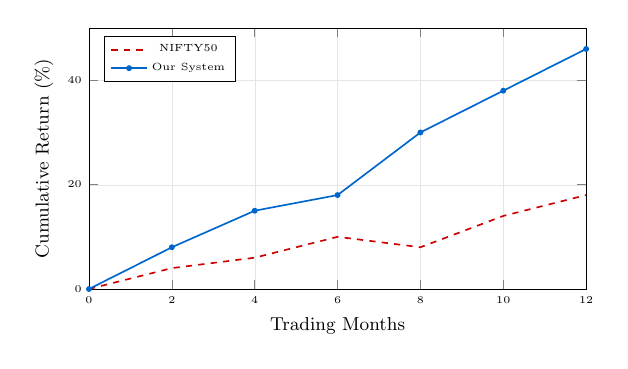
\begin{tikzpicture}[scale=0.75]
            \begin{axis}[
                width=10cm, height=6cm,
                xlabel={\small Trading Months},
                ylabel={\small Cumulative Return (\%)},
                xmin=0, xmax=12, ymin=0, ymax=50,
                legend pos=north west,
                legend style={font=\tiny, fill=white},
                grid=both,
                grid style={line width=.1pt, draw=gray!20},
                tick label style={font=\tiny},
            ]
            \addplot[color=AccentRed, thick, dashed] coordinates {
                (0,0)(2,4)(4,6)(6,10)(8,8)(10,14)(12,18)};
            \addlegendentry{NIFTY50}
            \addplot[color=IITBlue, thick, mark=*, mark options={scale=0.5}] coordinates {
                (0,0)(2,8)(4,15)(6,18)(8,30)(10,38)(12,46)};
            \addlegendentry{Our System}
            \end{axis}
            \end{tikzpicture}
            \end{center}
        \end{column}
    \end{columns}
\end{frame}

% 14. Conclusion
\section{Conclusion}
\begin{frame}{Conclusion}
    \begin{itemize}
        \item \textbf{It Works:} Reading the news with AI can reliably predict stock price movements.
        \item \textbf{Complete System:} We built a full working application — not just a script — with a live research dashboard.
        \item \textbf{Safety First:} Combining NLP alpha generation with mathematical risk optimization creates a strategy that is both profitable and controlled.
    \end{itemize}
\end{frame}

% 15. Future Work
\section{Future Work}
\begin{frame}{Future Work}
    \begin{itemize}
        \item \textbf{Twitter/X Integration:} Incorporating social media sentiment to catch rumors before they become news.
        \item \textbf{Intra-day Trading:} Shifting from daily OHLCV to minute-level tick data for faster signal capture.
        \item \textbf{LLM Summarization:} Using large language models to compress 50-page earnings transcripts into structured factor scores in seconds.
    \end{itemize}
\end{frame}

% 16. References
\section{References}
\begin{frame}{References}
    \begin{itemize}
        \item \textbf{Tetlock (2007):} Media pessimism predicts downward market pressure. \textit{Journal of Finance}.
        \item \textbf{Araci (2019):} FinBERT: Financial Sentiment Analysis with Pre-trained Language Models. \textit{arXiv:1908.10063}.
        \item \textbf{Markowitz (1952):} Portfolio Selection. \textit{Journal of Finance}, 7(1), 77--91.
    \end{itemize}
\end{frame}

\end{document}
